\section{机制检验与扩展策略比较}

\subsection{规划与执行偏差：一致性不等于低费用}

先固定原版参数，即12代表场景、自适应风险基数0.1及参考备用系数1，重建每个外层决策点的购电计划，再将相同历史场景输入原执行规则。重建购电量与保存轨迹在实际执行窗口完全一致。表\ref{tab:v2_execution_gap}汇总2月至12月决策点：问题二、三、四静态和四滚动的平均费用偏差分别为$-986.50$、$-569.90$、$-1068.47$和$-582.32$元，多数回放费用低于规划费用。

\begin{table}[htbp]\centering\small
\caption{原版同计划、同初态、同场景的规划与执行偏差}
\label{tab:v2_execution_gap}
\begin{tabularx}{\linewidth}{LRRRR}\toprule
问题 & 决策点数 & 平均$\Delta_{\rm exec}$/元 & 负偏差比例 & SOC均方根偏差/kWh\\\midrule
问题2 & 334 & -986.50 & 97.90\% & 1319.72\\
问题3 & 1336 & -569.90 & 94.24\% & 994.32\\
问题4-2 & 334 & -1068.47 & 99.40\% & 1350.69\\
问题4-3 & 1336 & -582.32 & 93.94\% & 1048.30\\
\bottomrule\end{tabularx}
\par\smallskip\parbox{\linewidth}{\footnotesize 每一决策点先按场景概率计算费用差与SOC均方根偏差，再对决策点取均值；滚动剩余时域相互重叠，不将这些差求和解释为年度费用。全部费用仅计实际结算项目。}
\end{table}

负偏差不表示规划正确描述了控制，而是参考储能在各场景共享，实际规则可利用当期观测调整动作，其实现费用可能更低。正偏差仍会出现。图\ref{fig:v2-gap}选取问题三正偏差最大决策点，展示不同场景下SOC偏离与费用差发生的时段。两条期望费用都仅计真实收费，不混入风险项或终端罚项；滚动剩余时域相互重叠，不能将这些偏差相加为年度节费。

\begin{figure}[htbp]\centering
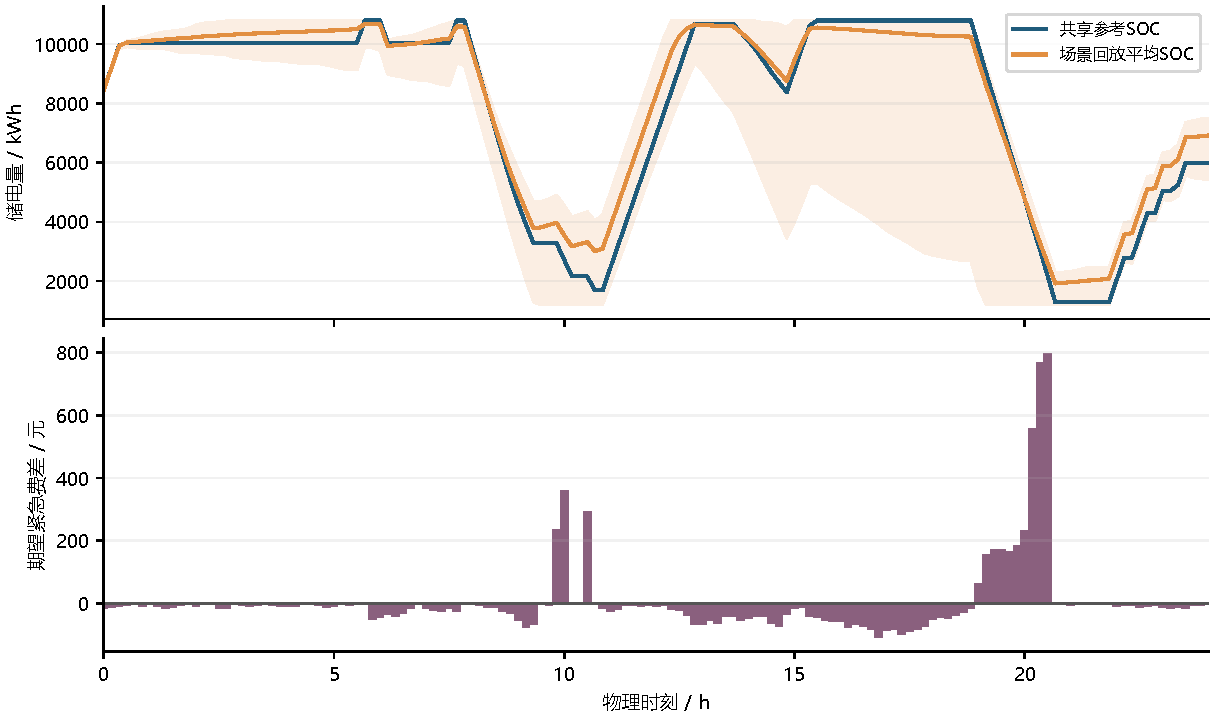
\includegraphics[width=0.96\linewidth]{figures/results/v2_execution_gap.pdf}
\caption{原版问题三正费用偏差最大决策点的参考与场景回放；阴影为回放SOC范围，费用差取回放减规划}\label{fig:v2-gap}
\end{figure}

进一步使用本次冻结的主案，在四个指定日的四个外层时点固定合同、初态及28场景，对规则执行和内层LP各回放448条轨迹。未来输入保持当时合法点预测，只有当前一步揭示场景净需求和价格，不读取未来场景实现或后续新预报。这样把“同计划下换控制器”的影响与“闭环运行导致后来计划也改变”的影响区分开来。

\begin{table}[htbp]\centering\small
\caption{未筛选母模型计划下两种执行器的回放诊断}
\label{tab:v2_inner_gap}
\begin{tabularx}{\linewidth}{LRR}\toprule
指标 & 规则执行 & 内层LP\\\midrule
有符号期望费用偏差/元 & -655.33 & -513.41\\
场景费用绝对偏差的期望/元 & 697.25 & 605.16\\
SOC均方根偏差/kWh & 1056.40 & 869.79\\
\bottomrule\end{tabularx}
\par\smallskip\parbox{\linewidth}{\footnotesize 四个指定日、四个时点共16个决策点，每点28场景。先计算场景概率加权指标，再对决策点等权平均；两种执行器固定相同购电合同和初态，仅逐步揭示当前场景值。}
\end{table}


内层LP将SOC均方根偏差均值由1056.40 kWh降至869.79 kWh，场景费用绝对偏差的期望由697.25元降至605.16元；但平均账单相对规则执行增加141.92元。16点中，绝对期望费用偏差在10点减小，实际回放账单仅1点更低。因而更接近参考轨迹是一项可观测改善，却不能替代经济目标。主案继续使用一月选中的执行规则，也承认其与上层场景评估尚未严格一致。

\subsection{风险与备用的单独贡献和联合作用}

题目已通过五倍补购价格计入应急代价，不另外要求紧急量达到某个阈值。表\ref{tab:v2_risk_modules}将期望费用、仅风险、仅备用及二者联合全部列出，风险与备用各比较固定和自适应版本。固定风险权重为一月匹配值0.10368，固定备用为208.67 kWh；二者都不根据评价期结果重新设定。

\begin{table}[htbp]\centering\small
\caption{问题2风险与备用的完整对照}
\label{tab:v2_risk_modules}
\begin{tabularx}{\linewidth}{LRRRR}\toprule
策略 & 总费/万元 & 紧急量/kWh & 日费CVaR95/元 & 末库存/kWh\\\midrule
期望费用 & 1401.28 & 85017.69 & 70731.74 & 6240.32\\
固定风险 & 1411.84 & 56316.17 & 69028.62 & 6318.65\\
自适应风险 & 1405.41 & 66920.81 & 69476.71 & 6255.33\\
固定备用 & 1401.09 & 74987.90 & 70409.51 & 6240.32\\
动态备用 & 1402.30 & 76168.28 & 70299.39 & 6245.11\\
固定风险+备用 & 1413.36 & 49102.47 & 68862.93 & 6318.65\\
自适应风险+备用 & 1406.93 & 59081.98 & 69070.96 & 6260.12\\
自适应联合，12场景 & 1404.26 & 75336.25 & 70065.84 & 6289.57\\
\bottomrule\end{tabularx}
\par\smallskip\parbox{\linewidth}{\footnotesize 本表基于未启用候选筛选的母模型，各组保留原实验配置及数值，覆盖相同334天并连续推进状态；不作为最终筛选算法的同条件消融。}
\end{table}

\begin{table}[htbp]\centering\small
\caption{固定与自适应策略在评价期实现的平均保守程度}
\label{tab:v2_conservatism}
\begin{tabularx}{\linewidth}{LRR}\toprule
策略 & 平均风险权重 & 平均参考备用/kWh\\\midrule
固定风险 & 0.10368 & 0.00\\
自适应风险 & 0.05506 & 0.00\\
固定备用 & 0.00000 & 207.22\\
动态备用 & 0.00000 & 244.39\\
固定联合 & 0.10368 & 207.22\\
自适应联合 & 0.05506 & 244.39\\
\bottomrule\end{tabularx}
\par\smallskip\parbox{\linewidth}{\footnotesize 固定参数由一月动态序列的均值匹配；由于季节与误差分布变化，评价期均值不保证相等，不用评价期重新匹配。}
\end{table}

问题二仅加固定风险或自适应风险分别多支付105631.25元和41280.51元，紧急量分别由85017.69 kWh降至56316.17和66920.81 kWh。固定备用单独使用节省1891.73元，动态备用单独使用增加10152.11元，效果并不统一。联合自适应策略比期望费用主案增加56524.93元，同时紧急量降至59081.98 kWh。这里控制的CVaR损失为紧急费用，实际日总费用尾部另列，不将两个对象混称。

固定与自适应之间的比较应结合平均保守程度。匹配在一月完成，评价期实际平均风险权重分别为0.103681与0.055059，参考备用分别为207.22与244.39 kWh，并未保持相等，故不能把全部费用差解释为“自适应识别风险的能力”。描述性联合交互项定义为$C_{\rm joint}-C_{\rm risk}-C_{\rm reserve}+C_{\rm expectation}$，固定及自适应两组分别为17088.03元和5092.30元。其为正表明本回测中联合使用比两项单独费用变化的线性叠加更贵，但这不是独立因果效应估计，也不是所有参数下都会重复保守的定理。

不以评价期最低费用的固定备用策略替换主案。风险控制回答的是“为减少昂贵补购或特定尾部损失，是否愿意支付额外费用”，应作为运行偏好扩展，而非赛题经济目标自动要求的内容。

\subsection{28日完整场景与12个代表场景}

28个等权历史日的10\%尾部仅有2.8条日轨迹的概率质量，少量样本已使CVaR估计不稳定。压缩成12个带权代表场景又可能把尾部集中到个别代表日。不能仅因两种场景数得出的总费用接近，就认定极端补购的形状也被保留。

\begin{table}[htbp]\centering\small
\caption{历史场景保留与缩减的经济对照}
\label{tab:v2_scenarios}
\begin{tabularx}{\linewidth}{LRRRR}\toprule
策略 & 总费/万元 & 紧急量/kWh & 日费CVaR95/元 & 末库存/kWh\\\midrule
问题2：28场景 & 1401.28 & 85017.69 & 70731.74 & 6240.32\\
问题2：12场景 & 1400.63 & 105407.24 & 72139.66 & 6257.26\\
问题3：28场景 & 1397.58 & 12647.76 & 65518.79 & 6240.32\\
问题3：12场景 & 1393.37 & 16150.68 & 65554.27 & 6271.05\\
\bottomrule\end{tabularx}
\par\smallskip\parbox{\linewidth}{\footnotesize 本表基于未启用候选筛选的母模型，各组保留原实验配置及数值，覆盖相同334天并连续推进状态；不作为最终筛选算法的同条件消融。}
\end{table}

\begin{table}[htbp]\centering\small
\caption{场景规模与每日平均运行时间}
\label{tab:v2_solve_times}
\begin{tabularx}{\linewidth}{LRR}\toprule
问题 & 场景数 & 秒/日\\\midrule
问题2 & 12 & 0.0276\\
问题2 & 28 & 0.0521\\
问题3 & 12 & 0.0699\\
问题3 & 28 & 0.1236\\
\bottomrule\end{tabularx}
\par\smallskip\parbox{\linewidth}{\footnotesize 运行时间含预测、外层求解与执行等开销，并行运行下的本机计时仅供工程量级参考。}
\end{table}

经济目标下，问题二12场景比28场景少付6465.72元，却多用20389.55 kWh紧急电量；问题三少付42065.07元，多用3502.93 kWh紧急电量。自适应风险与备用联合开启时，12场景费用14042623.21元、紧急量75336.25 kWh，28场景费用14069332.59元、紧急量59081.98 kWh，压缩对应的尾部账单与紧急需求发生明显变化。保留28场景没有保证评价期账单最小，但排除了额外的代表日压缩，其运行耗时仍适合本题规模，故按预定设置保留。28日历史本身的样本有限性仍然存在。

\subsection{储能LP和跨日价值的效果与边界}

\begin{table}[htbp]\centering\small
\caption{问题3母模型的执行控制与跨日续接对照}
\label{tab:v2_controllers}
\begin{tabularx}{\linewidth}{LRRRR}\toprule
策略 & 总费/万元 & 紧急量/kWh & 日费CVaR95/元 & 末库存/kWh\\\midrule
规则执行（母模型） & 1397.58 & 12647.76 & 65518.79 & 6240.32\\
剩余日储能LP & 1421.32 & 23825.27 & 66397.37 & 5934.55\\
储能LP+跨日价值 & 1405.26 & 22407.53 & 66033.05 & 6240.32\\
\bottomrule\end{tabularx}
\par\smallskip\parbox{\linewidth}{\footnotesize 本表基于未启用候选筛选的母模型，各组保留原实验配置及数值，覆盖相同334天并连续推进状态；不作为最终筛选算法的同条件消融。}
\end{table}


在完整闭环对照中，仅将问题三执行器改为剩余日LP，总费用为14213193.28元，比主案增加237382.42元，紧急量也增至23825.27 kWh。该结果与一月选型方向一致，不能为了形成“双时间尺度LP”的亮点而强行将其设为主方案。上层目标仍使用共享参考储能，内层仅依据有限预测近似后续价值，两者组合未必实现更低费用。

对相同LP控制器利用合法跨日预报后，总费用降至14052638.61元，比午夜截断的LP节省160554.67元，紧急量减少1417.74 kWh，年末库存还增加305.77 kWh，说明跨日信息改善并非通过更多放空电池取得。但它仍比规则主案多付76827.75元，不能据此宣称已经成为经济最优策略。

一个两时段例子说明内层LP的经济机制：电池具有1 kWh可对外输出的电量，两段常规合同均为0、净需求均为1 kWh，交易价格分别为1和2元/kWh，取消终端罚项。规则执行先放电，后一段补购支付10元；内层LP先支付5元补购、留电到后一段，账单为5元。程序验证了这一行为，但构造例子的机制优势不等于真实全年数据上的优势。

目前零时外层尚未显式建模以后1.5倍修订的机会，跨日续接也只是确定性临时购电价值。进一步改进宜在四个合法发布时点构造带非预见性约束的小场景树，或在上层直接评价同一因果控制策略。不能给各场景储能变量独立优化全天并称其为可执行方案，也不能把事后滚动重算等同于零时已经计入未来修订价值。

\subsection{结算解释的敏感性}

主口径不退款与取消部分退款的定义已在建模前列明。表\ref{tab:v2_settlement}固定本次问题三的预测、场景、控制器及初态，仅改变退款规则并重新优化，实际费用按各自规则结算。该对照用于暴露语义敏感性，不按哪种解释更便宜来选择主口径。主结果与附件5仍使用不退款规则。

\begin{table}[htbp]\centering\small
\caption{问题3母模型的结算解释敏感性}
\label{tab:v2_settlement}
\begin{tabularx}{\linewidth}{LRRRR}\toprule
策略 & 总费/万元 & 紧急量/kWh & 日费CVaR95/元 & 末库存/kWh\\\midrule
主口径：不退款 & 1397.58 & 12647.76 & 65518.79 & 6240.32\\
取消部分退款 & 1365.55 & 12871.85 & 64278.33 & 6240.32\\
\bottomrule\end{tabularx}
\par\smallskip\parbox{\linewidth}{\footnotesize 本表基于未启用候选筛选的母模型，各组保留原实验配置及数值，覆盖相同334天并连续推进状态；不作为最终筛选算法的同条件消融。}
\end{table}


退款解释下总费用13655463.35元，较主口径少320347.51元，累计下调1096916.99 kWh，净调整费用为$-113349.02$元。两组年末库存相同，费用差主要反映规则变化及对应采购响应，其量级大于若干模型增强的效果。该结果取代旧版参数下的退款数值，避免将不同版本的费用相减。

下调支配性始终依赖正电价、原计划不退款及免费弃余三个条件；退款口径改变取消计划的边际成本，下调量可以为正。解释敏感性与算法增强的费用差应分开报告，不能把制度变化形成的费用下降记为调度算法节费。

\section{模型评价与结论}

本文以收费机制、因果信息和物理状态为共同基础。单时段分位数推导解释非对称采购行为，完整LP处理储能容量、效率及跨时段竞争；所有实际账单由执行轨迹重新结算，规划偏差用同计划回放单独识别。主结果满足逐段能量平衡、容量与功率界、充放电互斥及跨日连续性。未来实际值和未来发布预报的扰动检查未改变已经执行的前缀，支持代码遵守所声明的信息时序。

仍需明确四项限制。第一，只有一个年度且一月校准窗口较短，修订已经参考过旧版回测结果，因此不能声称跨年份泛化或全新独立测试。第二，预测和控制采用有限候选的坐标搜索，额外风险与备用关闭等设置预先固定，并未穷举所有策略。第三，上层共享储能和实际控制之间仍有差异，未来修订机会、日际随机价值均未被精确求解。第四，终端惩罚是辅助近似，比较需同时报告末库存，且未引入赛题以外的网络限额、寿命退化或交易约束。

确定性条件下问题一费用35126.95元；不确定条件下，按五倍补购代价建立场景采购贡献了主要节费。问题二、三主费用分别1401.28万元、1397.58万元，动态电价两案分别1479.41万元、1476.92万元。风险、备用、内层LP和跨日续接的价值取决于实际数据与结算条件，不能预设复杂模型总是更优。本文的结论在于用收费结构解释决策，再用可复现账单判断各项增强是否值得保留。
